\documentclass[10pt,journal,compsoc]{IEEEtran}

\usepackage{verbatim}
\usepackage{url}
\usepackage{graphicx}

\usepackage{xspace}
\newcommand{\FC}       {Freechains\xspace}
\newcommand{\reps}     {\emph{reps}\xspace}
\newcommand{\onerep}   {\emph{1~rep}\xspace}
\newcommand{\nreps}[1] {\emph{#1~reps\xspace}}

\newcommand{\Xon} {$1{\rightarrow}N$\xspace}
\newcommand{\Xno} {$1{\leftarrow}N$\xspace}
\newcommand{\Xnn} {$N{\leftrightarrow}N$\xspace}
\newcommand{\Xoo} {$1{\leftrightarrow}1$\xspace}
\newcommand{\Xo}  {$1{\hookleftarrow}$\xspace}

\begin{comment}
- content                                                                       
- CPU work to create blocks, easy objective verification, 50+1 attack, collapse
- Human work to create content, easy subjective verification, 50+1 attack,
  community fork (actually encouraged)
- unique identity based on CPU
- here based on post quality
- not CDN: Content delivery network                                             

(b) double spend of coins/reps is solved by total ordering all
Users can like \& dislike posts, which transfer reputation between them.
Reputation is created from news

Just like Bitcoin reaches consensus with the longest chain
uses mining to

(excess, SPAM, fake, abuse, illegal)                                            
\end{comment}

\begin{document}
\title{
    Peer-to-Peer Consensus via Authoring Reputation
}
\author{
    %Francisco Sant'Anna~\IEEEmembership{Department of Computer Science, Rio de Janeiro State University}
}

\IEEEtitleabstractindextext{%
\begin{abstract}
Content publishing in public Internet forums and social media suffers from
excess and abuse, such as low quality posts and fake news.
Centralized platforms employ filtering algorithms and anti-abuse policies, but
impose full trust from users.
We propose a publish-subscribe peer-to-peer protocol to model public content
dissemination without centralized control.
The protocol mitigates abuse a reputation system that moderates content and, at
the same time, delivers network consensus.
We trace a parallel with Bitcoin:
    posts create reputation (vs proof-of-work),
    likes and dislikes transfer reputation (vs transactions),
    and aggregate reputation determines consensus (vs longest chain).
The reputation system depends solely on human work to create and rate content,
preventing abuse while imposing consensus on a peer-to-peer setting.
We prototype a simple permissionless version control system that relies on
reputation consensus to resolve conflicts automatically.
\end{abstract}

\begin{IEEEkeywords}
bitcoin, crdts, distributed consensus, peer-to-peer, publish-subscribe, reputation system, version control system
\end{IEEEkeywords}}

\maketitle

% TOTAL: 12 pages

\section{Introduction}
\label{sec.introduction}

\IEEEPARstart{C}{ontent} publishing in public Internet forums and social media
platforms is increasingly more centralized in the hands of a few
companies~\cite{internet.fixing,p2p.osn}.
%
On the one hand, these companies offer free storage, friendly user interfaces,
and robust access.
On the other hand, they concentrate more power than required to operate, since
they collect and control our data, ``algorithmize'' our consumption, and yet
obstruct portability with proprietary standards.
%
Peer-to-peer alternatives~\cite{p2p.survey} eliminate intermediaries and push
to end users the responsibility to manage data and connectivity.
However, due to decentralization of authority and network infrastructure, some
new challenges arise to deal with malicious users and enforce overall state
consistency.

In an ideal Internet forum, all messages or posts
(i)   reach even temporarily disconnected users;
(ii)  are delivered in a consistent order;
(iii) are respectful and on topic.
In a centralized system, items (i) and (ii) are trivially achieved assuming
availability and delivery order in the service, while for item (iii) users have
to trust the service to moderate content.
In a decentralized setting, however, none of these demands are easily
accomplished.
A common approach in gossiping protocols is to replicate the whole conversation
in all peers and disseminate it proactively until all users receive
it~\cite{p2p.survey}.
However, this approach does not guarantee consensus since posts can be received
in conflicting orders in different peers.
As an example, antagonistic messages such as \emph{"X is final"} vs
\emph{"Y is final"} might be sent concurrently, preventing the network to
determine as a group its intention as \emph{X} or \emph{Y}~\cite{p2p.intention}.

Bitcoin~\cite{p2p.bitcoin} proposes a permissionless consensus protocol founded
on scarce virtual assets, the \emph{bitcoin tokens}.
%
The only way to create new bitcoins is to work towards consensus in the network
by proposing a total order among all transactions in the system.
%
This way, Bitcoin prevents double spending~\cite{p2p.bitcoin}, which is
analogous to conflicting messages in public discussions:
    deciding between \emph{X} and \emph{Y} as a group is the same as
    transferring bitcoins to \emph{X} and \emph{Y} with insufficient funds for
    both.
%
However, Bitcoin just blindly transfers bitcoins between users, with no
subjective judgment that could affect the actual transactions.
In contrast, our challenge is to use social interactions between humans to
evaluate content and mitigate abuse.

In this work, we propose a consensus algorithm based on authoring reputation.
Inspired by Bitcoin, authors accumulate tokens named \reps, which serve as
currency to rate posts in the network.
Users can rate posts with likes and dislikes, which transfer \reps between
them.
Work is manifested as new posts which, if accepted by others, reward authors
with \reps.
This way, like Bitcoin, token generation is expensive, while verification is
cheap and made by multiple users.
However, unlike Bitcoin, both creation and verification are subjective, based
on human creativity and judgement, which match our target domain of content
publishing.
Posts and likes are linked as blocks in a Merkle~DAG that persists the whole
conversation and is disseminated in the network with gossiping.
To reach consensus, the DAG is sequenced as a linked list that orders branches
with more reputed authors first (i.e., branches with more work).
The list is then verified for conflicting operations, such as likes with
insufficient \reps, which is equivalent to double spending in Bitcoin.
In this case, the branch that causes the conflict, which is always the one with
less work, is removed from the DAG and the linked list is recalculated.
We integrated the proposed consensus algorithm into Freechains, a peer-to-peer
publish-subscribe content dissemination protocol~\cite{fcs.sbseg20}.
We also present the prototype of a permissionless version control system that
relies on consensus to apply automatic merges.

Our main contribution is to make public forums practical with complete
decentralization.
The proposed reputation and consensus mechanism depends solely on human work to
create and moderate content, which distinguishes itself from most systems which
rely on external resources to reach consensus.
The general idea of the algorithm can be applied to any public forum system
that uses DAGs to structure its messages.
%
As a main limitation, Merkle DAGs are ever growing data structures that also
carry considerable metadata overhead.
Pruning DAGs require particular solutions that do not solve the fundamental
problem.
%
Public forums are still social platforms and we do not claim that a reputation
system enforces ``good'' human behavior.
Instead, it provides a transparent and quantitative mechanism that helps users
understand the evolution of the community and act accordingly.

\begin{figure*}
\centering
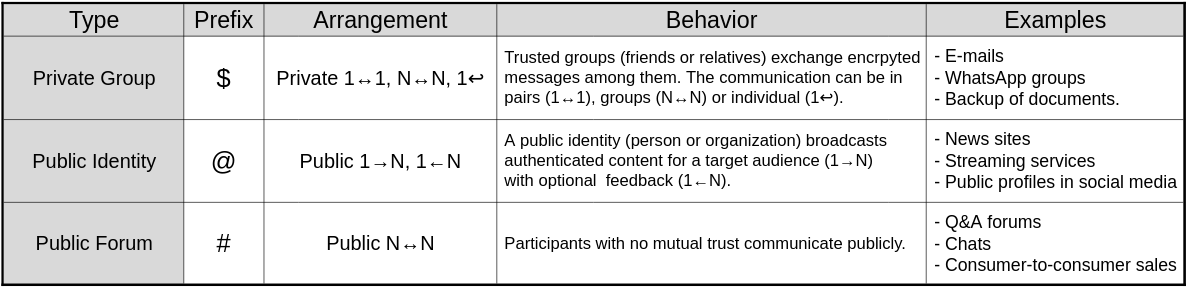
\includegraphics[width=\textwidth]{arrangements.png}
\caption{The three types of chains and arrangements in \FC.}
\label{fig.table}
\end{figure*}

In Section~\ref{sec.freechains}, we introduce the basic functionalities of \FC
to create, rate, and disseminate posts.
In Section~\ref{sec.consensus}, we describe the general reputation and
consensus mechanism, and how it integrates with public forums in \FC.
In Section~\ref{sec.crdts}, we discuss the correspondences with CRDTs and
present the version control system prototype.
In Section~\ref{sec.related}, xxx.
In Section~\ref{sec.conclusion}, yyy.

\section{Freechains}
\label{sec.freechains}

\FC is an unstructured peer-to-peer topic-based publish-subscribe
system~\cite{fcs.sbseg20}.
Each topic, or \emph{chain}, is organized as a \emph{Merkle DAG}, i.e., a
directed acyclic graph immune to modifications.
The chain DAG is disseminated peer by peer in the network with gossiping.
This way, as an author posts to a chain, other users subscribed to the same
chain eventually receive the message.
\FC supports multiple types of chains with different arrangements of public and
private communication, which are detailed in Figure~\ref{fig.table}.
In this section, we operate a private group to describe the basic behavior of
chains.
At the end of the section, we also exemplify a public identity chain.
In Section~\ref{sec.consensus}, we detail the behavior of public forums, which
involve untrusted communication between users and require the proposed
reputation and consensus mechanism.

All \FC operations go through a \emph{daemon} (analogous to Bitcoin full nodes)
which validates posts, links them in the Merkle DAGs, persists the chains in
the disk, and communicates with other peers in the network to disseminate the
graphs.
The command that follows starts a daemon to serve further operations:

{\footnotesize
\begin{verbatim}
 > freechains-daemon start '/var/freechains/'
\end{verbatim}
}

The actual chain operations use a separate client to communicate with the
daemon.
The next sequence of commands (i) creates a shared key, (ii) joins a private
group chain (prefix $\$$), and (iii) posts a message into the chain:

{\footnotesize
\begin{verbatim}
 > freechains crypto shared 'strong-password' # (i)
 A6135D..   <- returned shared key
 > freechains '$family' join 'A6135D..'       # (ii)
 42209B..   <- hash of chain
 > freechains '$family' post 'Good morning!'  # (iii)
 1_EF5DE3.. <- hash of post
\end{verbatim}
}

\begin{figure}
\centering
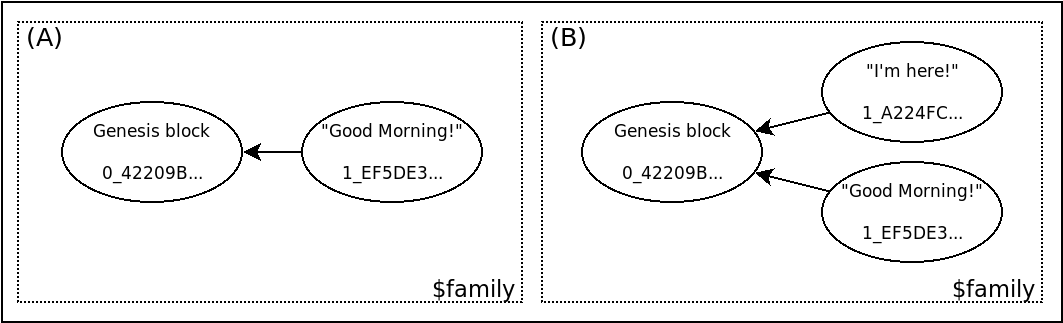
\includegraphics[width=0.5\textwidth]{family.png}
\caption{Two DAG configurations. (A) has a single head pointing to the
genesis block. (B) has a fork with two heads pointing to the genesis block.}
\label{fig.family}
\end{figure}

A private chain requires that all participants use the same shared key to join
the group.
A \emph{join} only initializes the DAG locally in the file system, and a
\emph{post} also only modifies the local structure.
No communication occurs at this point.
Figure~\ref{fig.family}.A depicts the state of the chain after the first post.
The genesis block with height $0$ and hash \texttt{42209B..}
depends only on the arguments given to \emph{join}.
The next block with height $1$ and hash \texttt{EF5DE3..} contains the posted
message.
As expected from a Merkle~DAG, the hash of a block depends on its payload and
hash of previous block.

\FC adheres to the \emph{local-first} software principle~\cite{p2p.local},
allowing networked applications to host their own data and work locally while
offline.
Except for synchronization, all other operations in the system only affect the
local replica.
In particular, joining a chain with the same arguments in another peer results
in the same genesis state, even if the peers have never met before.
Hence, before synchronizing, others peers have to initialize the example chain
with the same steps:

{\footnotesize
\begin{verbatim}
 > freechains-daemon start '/var/freechains/'
 > freechains crypto shared 'strong-password'
 A6135D..
 > freechains '$family' join 'A6135D..'
 42209B..
\end{verbatim}
}

Synchronization is explicit, in pairs, and unidirectional.
The command \emph{recv} asks daemon in \emph{localhost} to connect to daemon in
\emph{remote-ip} and receive all missing blocks from there:

{\footnotesize
\begin{verbatim}
 > freechains '$family' recv '<remote-ip>'
 1/1  <- one block received from <remote-ip>
\end{verbatim}
}

The complementary command \emph{send} synchronizes the DAGs in the other
direction.
Note that \FC does not construct a network topology or synchronize peers
automatically.
There are no preconfigured peers, no root servers, no peer discovery.
All connections happen through the \emph{send} and \emph{recv} commands which
have to specify the peers explicitly.
In this sense, the protocol only gives basic support for communication in pairs
of peers and any further automation requires external tools.

The next sequence of commands checks the hash(es) of the block(s) at the head
of the local DAG (the latest blocks), and then reads the payload of the single
head found:

{\footnotesize
\begin{verbatim}
 > freechains '$family' heads
 1_EF5DE3..
 > freechains '$family' payload '1_EF5DE3..'
 Good morning!
\end{verbatim}
}

Now, the new peer is in the same state as the original peer in
Figure~\ref{fig.family}.A.
However, since the network is inherently concurrent and users are encouraged to
work locally, typical graphs are not lists, but DAGs with multiple heads.
As an example, suppose the new peer posts a message "I'm here!" \textbf{before}
the \emph{recv} above, when the local DAG is still in its genesis state.
In this case, as illustrated in Figure~\ref{fig.family}.B, the resulting graph
after the synchronization now contains two blocks with height $1$.
%
Note that forks in the DAG create ambiguity in the order of messages, which is
the fundamental obstacle to reach consensus.
In private chains, which we use in this example, we can apply simple methods to
reach consensus, such as relying on the timestamps of blocks.
However, in public forums, a malicious user can modify his local time to affect
new block timestamps and manipulate the order of messages.

To conclude the basic chain operations, users can rate posts with \emph{likes}
and \emph{dislikes}, which can be consulted later:

{\footnotesize
\begin{verbatim}
 > freechains '$family' like '1_EF5DE3..'
 2_BF3319..
 > freechains '$family' reps '1_EF5DE3..'
 1  # post received 1 like
\end{verbatim}
}

In private groups, likes are unlimited and behave much like typical centralized
systems.
In public forums, however, likes are restricted, have to be signed by users,
and are at the core of the consensus algorithm.

For the sake of completeness, \FC also supports public identity chains (prefix
$@$), which relies on public-key cryptography to attach an identity to a chain
and verify the authenticity of posts:

{\footnotesize
\begin{verbatim}
 > freechains crypto pubpvt 'other-password'
 EB172E.. 96700A..   <- public and private keys
 > freechains '@EB172E..' join
 F4EE21..
 > freechains '@EB172E..' post 'This is Pele' \
    --sign='96700A..'
 1_547A2D..
\end{verbatim}
}

In the example, a public figure creates a pair of public/private keys and joins
an identity chain attached to his public key.
Every post in this chain needs to be signed with the associated private key to
be accepted in the network.

\FC is less than $1500$ LoC in Kotlin and is publicly
available~\footnote{\url{http://www.freechains.org}}.
The binary for the JVM is less than $6Mb$ in size and works in Android and most
desktop systems.

\section{Reputation and Consensus Mechanism}
\label{sec.consensus}

In the absence of moderation, peer-to-peer public forums are impractical.
At the root of the problem lies Sybil attacks, which use large numbers of fake
identities to abuse the system.
For instance, it should take a few seconds to generate thousands of
public/private key identities and SPAM million of messages into the system.
%Hence, without moderation, there are no limits on the number and size of posts
%and no reasonable policy to distinguish quality.
For this reason, we propose a reputation system that works together with a
consensus algorithm to mitigate Sybil attacks and make peer-to-peer public
forums practical.

Section~\ref{sec.consensus.design} describes the overall reputation and
consensus mechanism, which can be applied to any public forum system that uses
DAGs to structure its messages~\cite{33,34,p2p.merkle-crdts}.
Section~\ref{sec.consensus.chains} describes the concrete rules we implement
for public forums in \FC.

\subsection{Overall Design}
\label{sec.consensus.design}

In the proposed reputation system, users can spend tokens named \reps to post
and rate content in the forums:
a \emph{post} operation initially penalizes authors until it consolidates and
counts positively;
a \emph{like} operation is a positive feedback that helps subscribers
distinguish good content amid excess;
a \emph{dislike} operation is a negative feedback that revokes content when
crossing a threshold.
Figure~\ref{fig.general} summarizes the reputation operations and their goals.
%
However, without restrictions, posts and likes alone are not satisfactory in
the presence of Sybils.
Therefore, \reps must be subject to some sort of scarcity that demands
non-trivial work immune to automation.

\begin{figure}
\centering
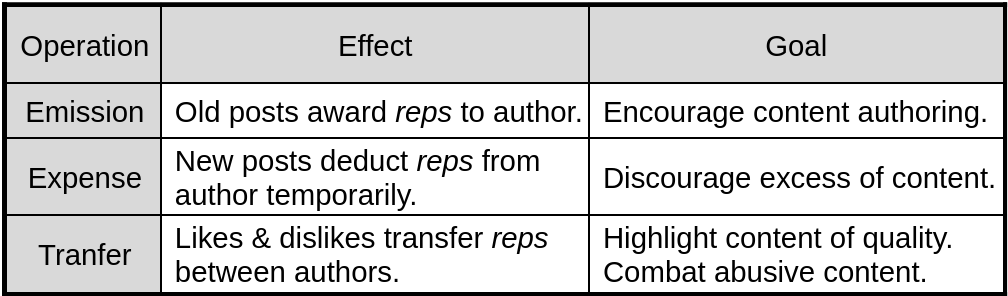
\includegraphics[width=0.49\textwidth]{general.png}
\caption{General reputation operations in public forums.}
\label{fig.general}
\end{figure}

Bitcoin employs CPU proof-of-work to mitigate Sybil attacks.
However, in the context of content publishing, we understand that authoring is
already an intrinsic human work that we can take advantage.
Creating new content is hard and takes time, but is comparatively easy to
verify and rate.
Therefore, in order to impose scarcity, only content authoring generates \reps,
while likes and dislikes only transfer \reps between users.
%but limited by periods of time to prevent excess (e.g., once in a day per user).
%Additionally,
%
Still, scarce posts and likes are not yet enough because they demand consensus
in the network.
Now, we need to track the reputation of users to check if they are allowed to
post new messages or spend likes.
Since posts and likes are concurrent in the network, we need to figure out how
to order them consistently across all peers so that they converge to the same
state.
As an example, it is possible that an author with a single unit of \reps
receives a dislike at the same time he posts a new message in the network.
If accounted before, the dislike blocks the new post, otherwise the post is
valid.
Even though it is impossible to determine which action happened first, the
network as a whole needs to agree on a single order because this decision
affects all future operations.

\begin{figure}
\centering
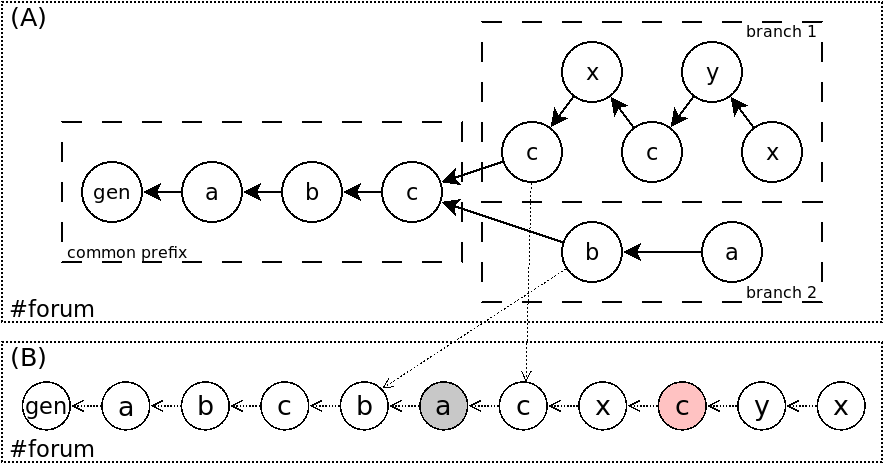
\includegraphics[width=0.49\textwidth]{reps2.png}
\caption{
    (A) A public forum DAG with a common prefix and two branches.
    (B) Total order between blocks of the DAG.
}
\label{fig.reps}
\end{figure}

Our solution is to order posts in the network favoring forks with participants
that constitute the majority of reputation.
This way, in order to manipulate consensus, malicious users first need to
cooperate to gain reputation, which is a non-trivial work and contradicts their
intent.
%
Figure~\ref{fig.reps}.A illustrates the reputation criterion.
%, still abstractly, since we did not discuss the actual rules for content creation and rating.
A public forum DAG has a common prefix with signed posts from users $a$, $b$,
and $c$.
Let's assume that within the prefix, users $a$ and $b$ have contributed with
better content and have more reputation combined than $c$ has alone.
%
After the prefix, the forum forks in two branches:
in \emph{branch~1}, only user $c$ remains active and we see that new users $x$
and $y$, with no previous reputation, generate a lot of new content;
in \emph{branch~2}, only users $a$ and $b$ participate but with less activity.
Nonetheless, \emph{branch~2} takes priority because, before the forking point,
$a$ and $b$ have more reputation than $c$, $x$, and $y$ combined.
%
User $c$ here represents a malicious user trying to cultivate fake identities
$x$ and $y$ in separate of the network to accumulate \reps.
However, the whole malicious \emph{branch~1} is vulnerable because users in
\emph{branch~2} with more previous reputation take the priority and can
overthrow user $c$.

Figure~\ref{fig.reps}.B indicates the consensus order between blocks in the
forum.
All operations in \emph{branch~2} are accounted before any operation in
\emph{branch~1}.
%
At any point in the consensus timeline, if an operation fails, all remaining
blocks in the offending branch are removed from the forum DAG.
As an example, suppose the last post by $a$ (in gray) is a dislike to user $c$,
which decreases its reputation.
Then, it's possible that the last post by $c$ (in red) is rejected together
with all posts by $y$ and $x$ in sequence.
Note that in a Merkle DAG, it is not possible to remove only the block with the
failing operation.
We need to remove the whole remaining branch as if it never existed.
%
Unlike Bitcoin, forks are not only allowed but encouraged due to the
local-first principle.
The resulting ordered list is only a view of the primary DAG structure.
However, the longer a peer remains disconnected, the more conflicting
operations it may perform, and the higher are the chances of rejection when
rejoining.
%
Note that users in \emph{branch~2} with more reputation may judge
\emph{branch~1} as malicious and can react even after the fact.
For instance, users $a$ and $b$ can post extra dislikes in \emph{branch~2} so
that merging with \emph{branch~1} removes all of its blocks.

Some other considerations about merging forks:
Peers that received branches with less reputation first (\emph{branch~1}) will
need to reorder all blocks starting at the forking point.
This might even involve removing content in the end user software.
This behavior is similar to blockchain reorganization in Bitcoin when a peer
detects a new longest chain and disconsiders old blocks.
%
Likewise, peers that saw branches with more reputation first (\emph{branch~2})
just need to put the other branch in sequence and do not need to recompute
anything.
This should be the normal behavior and is expected to happen in the majority of
the network.

\begin{figure}
\centering
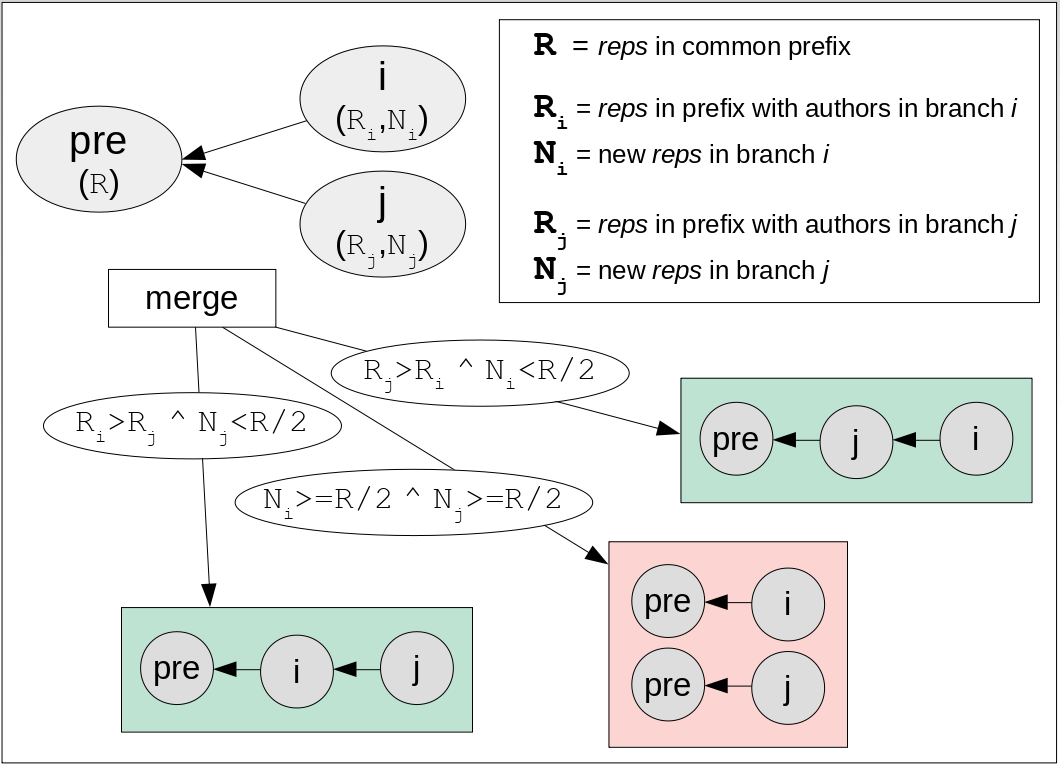
\includegraphics[width=0.49\textwidth]{merge.png}
\caption{
    Merging rules:
    (a) The branch with more reputation in the common prefix is ordered first.
    (b) A branch with 50\% or more reputation then its prefix is ordered first.
    (c) The merge fails if rules (a) and (b) conflict.
}
\label{fig.merge}
\end{figure}

As a counterpoint, suppose users $a$ and $b$ in Figure~\ref{fig.reps}.A have
actually abandoned the chain for months and thus \emph{branch-1} is legit.
In this case, $a$ and $b$ are the ones trying to take over the chain by
forging an early \emph{branch-2}, even with knowledge about \emph{branch-1}.
There is even a third option in which both branches are legit but became
disconnected for a long period.
It is impossible to determine.
Nonetheless, the breach that permits an forged branch to take over a long
active chain is compromising.
For this reason, the consensus algorithm includes an extra constraint when
merging:
If a branch creates new \reps that reach $50\%$ of its prefix, then the
algorithm guarantees that this branch takes priority in merges.
In the example, suppose that the common prefix accumulates \nreps{50}
considering users $a$, $b$, and $c$.
If \emph{branch-1} creates at least $25$ new \reps, then the merge with
\emph{branch-2} will fail and the chains will never synchronize again.
This situation is analogous to a hard fork in Bitcoin.
%
Figure~\ref{fig.merge} summarizes the merging algorithm:
    rule (a) favors the branch with more reputation;
    rule (b) forces the branch with $50\%+$ \reps of its prefix to go first;
    rule (c) enforces that previous rules do not conflict.

A fundamental drawback of Merkle DAGs is that all replicas in the system need
to store the complete graph in order to synchronize and verify new blocks.
Tree pruning techniques allow to remove parts of the graph to save
space~\cite{p2p.prune}.
The rule (b) in the consensus algorithm allows to prune the chain DAG, at least
for lightweight clients for resource-constrained devices.
A branch that reaches the threshold of $50\%+$ \reps is freezed in the ordered
list and becomes safe to remove along with all of its past back to the genesis
block.
However, this host can no longer verify forks starting past the removed blocks
and will fail to synchronize.
In this case, the host needs to delegate trust to other nodes for the first
verification of these forks.

\subsection{Public Forum Chains}
\label{sec.consensus.chains}

\begin{figure*}
\centering
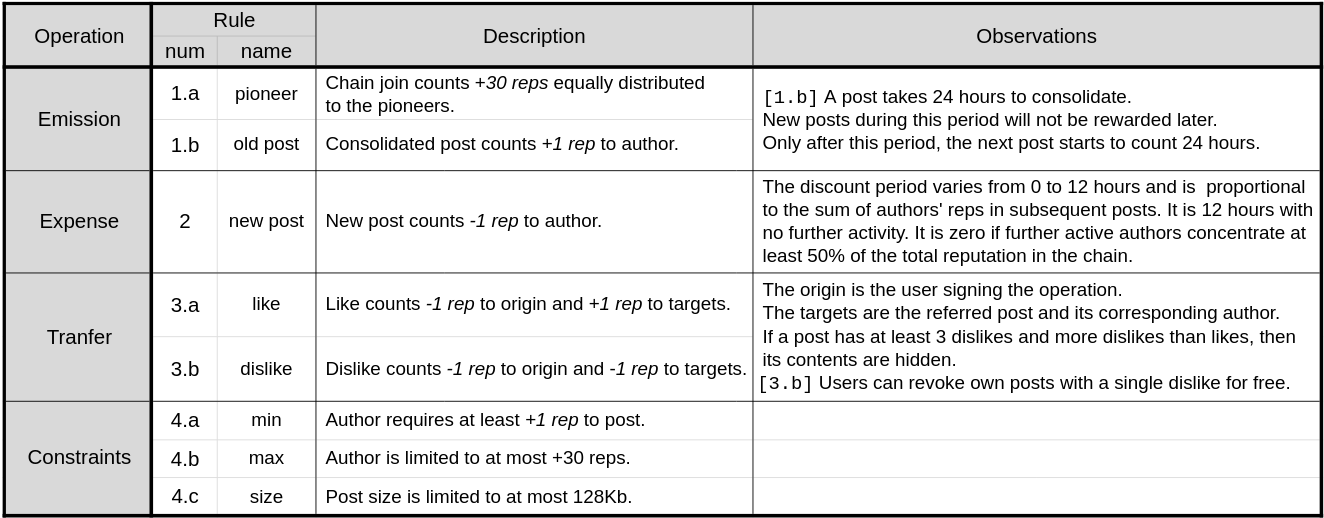
\includegraphics[width=\textwidth]{rules.png}
\caption{Specific reputation rules for public forum chains in \FC.}
\label{fig.rules}
\end{figure*}

We integrated the proposed reputation system in the public forums of \FC to
support content moderation and enforce consensus in the chains.
Figure~\ref{fig.rules} details the concrete rules which are discussed as
follows.
Authors have to sign their posts in order to be accounted by the reputation
system and operate in the chains.
The example that follows creates an identity whose public key is assigned as
the pioneer in a public chain (prefix $\#$):

{\footnotesize
\begin{verbatim}
 > freechains crypto pubpvt 'pioneer-password'
 4B56AD.. DA3B5F..
 > freechains '#forum' join '4B56AD..'
 10AE3E..
 > freechains '#forum' post --sign='DA3B5F..' \
    'The purpose of this chain is...'
 1_CC2184..
\end{verbatim}
}

The \emph{join} command in rule~\texttt{1.a} bootstraps a public chain,
assigning \nreps{30} equally distributed to the pioneers referred in the public
keys.
The pioneers shape the initial culture of the chain with its first posts and
likes, while he gradually transfers \reps to other authors, which may also
transfer to other authors, expanding the community.
%
In this regard, the \emph{post} command in sequence, which is signed by the
single pioneer and indicates the purpose of the chain to future users.

Our most basic concern in public forums is to resist Sybils spamming the
chains.
Fully peer-to-peer systems cannot rely on identity logins or CAPTCHAs due
to the lack of a central authority.
Other alternatives include (i) building social trust graphs, in which users
already in the community vouch for new users, or (ii) imposing economic costs
for new posts, such as proof of work.

We propose a mix between trust graphs and economic costs.
Rule~\texttt{4.a} imposes that authors require at least \onerep to post, while
rule~\texttt{2} imposes a cost of \onerep for each new post.
To vouch for new users, rule~\texttt{3.a} allows that existing users like and
unblock newbies' posts, but also at the cost of \onerep.
These rules impose costs not only for welcoming new users, but also for posting
new messages, which prevents abuse from malicious users already in the chain.
%
Note that the pioneer rule~\texttt{1.a} solves the chicken-and-egg problem
imposed by rule~\texttt{4.a}.

The next commands illustrate the reputation rules with numbers.
A new user joins the same public chain as before and posts a message, which is
welcomed with a like signed by the pioneer:

{\footnotesize
\begin{verbatim}
 > freechains crypto pubpvt 'new-author-password'
 503AB5.. 41DDF1..
 > freechains '#forum' join '4B56AD..'
 10AE3E..  <-- same pioneer as before
 > freechains '#forum' post 'Im a newbie...' \
    --sign='41DDF1..'
 2_C3A40F..
 > freechains '#forum' like '2_C3A40F..' \
    --sign='DA3B5F..'
 3_59F3E1..
\end{verbatim}
}

Note that chains with the same name but different pioneers are incompatible
because the hash of genesis blocks also depend on the pioneers' public keys.

\begin{figure}
\centering
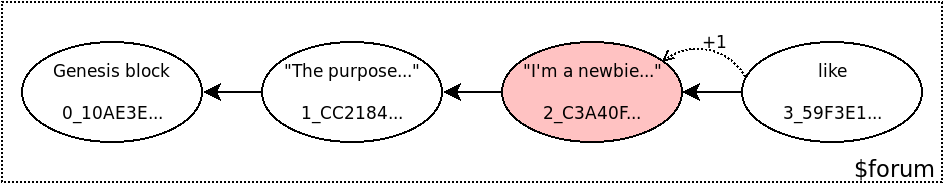
\includegraphics[width=0.49\textwidth]{forum.png}
\caption{
    The \texttt{like} approves the newbie message into the \texttt{\#forum} DAG.
}
\label{fig.forum}
\end{figure}

Figure~\ref{fig.forum} illustrates the chain DAG up to the like operation.
The pioneer starts with \nreps{30} (rule~\texttt{1.a}) and posts an initial
message.
%
A new post penalizes its author with \nreps{-1} (rule~\texttt{2}) which is
restored after at most 12 hours.
This period depends on the activity that comes after the new post (including
it).
The more activity from reputed authors, the less time the discount persists.
In the example, since the post is from the pioneer, which currently controls
all \reps in the chain, the penalty falls immediately and the pioneer remains
with \nreps{30}.
This mechanism limits the excess of posts in a chain dynamically.
For instance, in a slow technical mailing list, it is more expensive to post
messages in sequence.
However, in a chat with the majority of users participating, the penalty for
new posts can be reduced to zero.
%
Back to the figure, a new user with \nreps{0} tries to post a message
(hash~\texttt{C3A40F..}), which is initially blocked (rule~\texttt{4.a}), as
the red background highlights.
Then, the pioneer likes the blocked message, which reduces himself to
\nreps{29} and increases new user to \onerep (rule~\texttt{3.a}).
Once again, the penalty expires immediately since the like that follows the new
post is from the pioneer still with all \reps in the chain.
%
\begin{comment}
At the end, the pioneer has \nreps{28} and the new user remains with \nreps{0}
but with his post accepted.
Note that the overall balance after the commands is -\nreps{2} due to the
penalties of the two post operations (rule~\texttt{2}).
After at most 12 hours, these penalties are dismissed and the \nreps{2} are
recovered (rule~\texttt{2}):
    the pioneer goes to \nreps{29} and the new user to \onerep, which sum up to
    the pioneer's original \nreps{30}.
\end{comment}
%
With no additional rules to generate \reps, the initial \nreps{30} would
constitute the whole ``chain economy'' forever.
For this reason, rule~\texttt{1.b} awards authors 24 hours after each new post
with \onerep.
This rule stimulates content creation and grows the economy of chains.
The 24-hour period allows other users to judge the post before awarding its
author, and also regulates the growth speed of the chain.
Therefore, after the commands above complete 1 day, the pioneer accumulates
\nreps{30} and the new user \nreps{2}, growing the economy in \nreps{2} as
result of the two consolidated posts.
Note that rule~\texttt{1.b} awards at most one post at a time.
New posts during the 24-hour period will not awards extra \reps to the author.
Note also that rule~\texttt{4.b} limits authors to at most \nreps{30}, which
provides incentives to spend likes and thus decentralize the network.

Likes and dislikes (rules \texttt{3.a} and \texttt{3.b}) serve three purposes
in the chains:
    (i) welcoming new users,
    (ii) measuring the quality of posts, and
    (iii) censoring abuse (SPAM, fake news, illegal content).
%
The reputation of a given post is the difference between its likes and
dislikes, which can be used in end-user software for filtering and highlighting
purposes.
%
The quality of posts is subjective and is up to users to judge then with likes,
dislikes, or simply abstaining.
On the one hand, since \reps are finite, users need to ponder to avoid
indiscriminate expenditure.
On the other hand, since \reps are limited to at most \nreps{30} per author
(rule~\texttt{4.b}), users also have incentives to rate content.
Hence, the scarcity and limits work together towards the quality of the chains.
%
Note that a dislike shrinks the chain economy since it removes \reps from both
the origin and target.
As detailed next, the actual contents of a post may become hidden if it has at
least 3 dislikes and the number of dislikes is higher than the number of likes
(rule~\texttt{3}).
However, considering that \reps are scarce, dislikes should be more directed to
combat abuse, but not much to eliminate divergence of opinion.

\begin{figure}
\centering
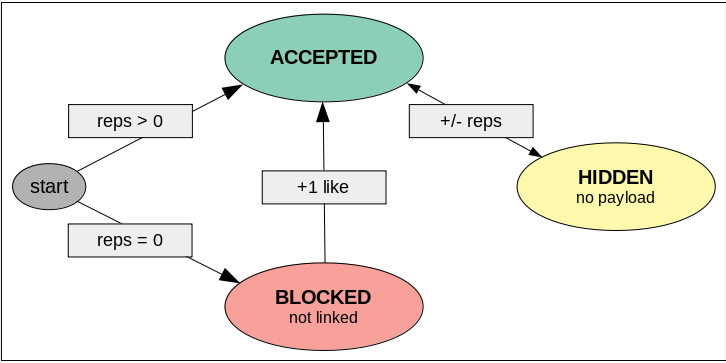
\includegraphics[width=0.49\textwidth]{state.png}
\caption{
    State machine of posts:
    \emph{BLOCKED} posts are not linked in the DAG.
    The payload of \emph{HIDDEN} posts are not retransmitted.
    \emph{ACCEPTED} posts are linked and retransmitted.
}
\label{fig.state}
\end{figure}

A post has three possible states: \emph{BLOCKED}, \emph{ACCEPTED}, or
\emph{HIDDEN}.
Figure~\ref{fig.state} specifies the transitions between the states.
%
If the author has reputation, its new post is immediately \emph{ACCEPTED} in
the chain.
Otherwise, it is \emph{BLOCKED} and requires a like from another user.
Blocked posts are not considered part of the chain DAG in the sense that new
posts do not link back to it.
%
Peers are not required to hold blocked posts and neither retransmit them to
other peers.
However, if blocked posts do not reach other users, they will never have the
chance to be welcomed with a like.
A reasonable policy for blocked posts is to hold them in a temporary bag and
retransmit them for some visibility in the network.
Rule~\texttt{4.c} limits the size of posts to at most \emph{128Kb} to prevent
DDoS attacks using gigantic blocked posts.
%
Once accepted, a post becomes part of the chain and can never be removed
again since Merkle DAGs are immutable by design.
%Note that blocked posts that become accepted are always succeeded by a
%\emph{like} (Figure~\ref{fig.forum}).
%
If the number of dislikes of a post exceeds the threshold (rule~\texttt{3}),
its payload becomes \emph{HIDDEN} and is not retransmitted to other peers.
% and should be removed from local storage.
Since the Merkle DAG depends only on its hash, removing the actual payload is
harmless.
Also, the DAG itself contains the dislikes that prove the hidden state to other
peers.
Later, if the post receives new likes and changes its state, it means that the
payload is still known somewhere and peers can request it when synchronizing
again.

\section{Correspondence with CRDTs}

Conflict-free replicated data types (CRDTs) are data structures that can be
updated concurrently with the guarantee that they converge to the same state on
synchronization, despite arbitrary failures~\cite{p2p.crdts}.
%
CRDTs serve as a robust foundation to model data in networked local-first
applications~\cite{p2p.local}.

Considering \FC operating as a transport layer for networked applications, the
Merkle DAG chains are trivially CRDTs because the DAG itself is the
CRDT~\cite{p2p.merkle-crdts}.
More specifically, they are state-based CRDTs (CvRDTs) because, on
synchronization, the missing parts of the self-verifiable DAGs are exchanged to
converge to the same state.
%
At the application layer, however, DAGs are not CRDTs because branches are
delivered to peers in different orders, and thus can lead to different states
when processed.
An interesting approach~\cite{p2p.merkle-crdts} is to require blocks in the
DAGs to represent commutative operations.
Commutative operations, combined with Merkle's exactly-once delivery guarantee,
lead to operation-based CRDTs (CmRDTs) at the application layer.
CmRDTs have the advantage that it only needs to store the operations to
reconstruct any version of the data, instead of storing each complete version
of the data as required in CvRDTs.
%
Our proposed consensus algorithm goes one step further and transforms a DAG
into a totally-ordered set, which leads to a CRDT that does not require
commutative operations.

Next, we illustrate the three-layered CRDT framework through an example of a
simple permissionless peer-to-peer Version Control System implemented on top
of public chains.

\subsection{A P2P VCS with Automatic Merge}

We built a simple peer-to-peer Version Control System with the following
operations and respective \FC operations in parenthesis:
%
\begin{itemize}
    \setlength{\itemindent}{-8pt}
    \item initialize a repository (\texttt{join})
    \item commit local changes to repository (\texttt{post})
    \item checkout repository changes to local (\texttt{traverse/payload})
    \item synchronize with remote peer (\texttt{send/recv})
    \item rate commits with likes \& dislikes (\texttt{like/dislike})
\end{itemize}
%
The system executes under public chains, which means that repositories are
permissionless and adhere to the reputation and consensus mechanism of \FC.
The main innovations in this system are that
    (i)  users can rate commits which can thus be rejected,  and
    (ii) checkouts merge commits automatically based on consensus.

Suppose we want to model a Wiki with public forums in \FC.
Each article is a chain behaving as its own VCS, holding the full edition
history.
Articles can link to other articles referring to other chains.

We use the \FC operations directly, except for \emph{commit} and
\emph{checkout}, which require multiple operations.
As an example, we join a public chain with the name of the file we want to
track and multiple pioneers.
We then edit the file and commit it:

{\footnotesize
\begin{verbatim}
 > freechains #p2p.md join A2885F.. 2B9C32..
 > echo "Peer-to-peer networking is..." > p2p.md
 > freechains-vcs #p2p.md commit --sign=699299..
 1_4F3EE1..
 > echo "The [USENET](#usenet.md), ..." >> p2p.md
 > freechains-vcs #p2p.md commit --sign=699299..
 2_B58D22..
\end{verbatim}
}

The \emph{commit} operation expands as follows:

{\footnotesize
\begin{verbatim}
 > freechains-vcs #p2p.md checkout p2p.remote
 > diff p2p.remote p2p.md > p2p.patch
 > freechains #p2p.md post p2p.patch --sign=699299..
\end{verbatim}
}

A commit first checks out the remote version held in the chain to an output
file \texttt{p2p.remote}.
Then, it diffs the remote against the local version to generate the file
\texttt{p2p.patch} with our changes.
Finally, the commit posts the signed patch file into the chain.

Much time later, another reputed author synchronizes with us, checks out the
file, then edits and commits it back:

{\footnotesize
\begin{verbatim}
 > freechains #p2p.md recv '<our-ip>'
 > freechains-vcs #p2p.md checkout p2p.md
 > echo "Peer-to-Peer does not scale!" >> p2p.md
 > freechains-vcs #p2p.md commit --sign=320B59..
 23_AE3A1B..
\end{verbatim}
}

The checkout operation needs to recreate the file by applying all patches since
the genesis block:

{\footnotesize
\begin{verbatim}
 > rm p2p.md && touch p2p.md
 > for blk in `freechains #p2p.md traverse` do
     freechains #p2p.md payload $blk > p2p.patch
     patch p2p.md p2p.patch
     if [ $? != 0 ]; then
       echo $blk  # hash of failing patch
       break
     fi
   done
\end{verbatim}
}

The \texttt{traverse} operation returns all hashes since the genesis block
respecting the consensus order.
The loop reads each of the payloads representing the patches and apply them in
order to recreate the current version of the file in the chain.
If the patch application fails, the command exhibits the hash of the block in
the screen.

Since the last edition is clearly wrong, other users in the network will
dislike its commit until it becomes \emph{HIDDEN} in the chain (as described in
Figure~\ref{fig.state}):

{\footnotesize
\begin{verbatim}
 > freechains #p2p.md dislike 23_AE3A1B.. --sign=USR1
 > freechains #p2p.md dislike 23_AE3A1B.. --sign=USR2
 > freechains #p2p.md dislike 23_AE3A1B.. --sign=USR3
 > freechains-vcs #p2p.md checkout p2p.md
 > cat p2p.md
 Peer-to-peer networking is...
 The [USENET](#usenet.md), ...
 ...
\end{verbatim}
}

This way, the checkout operation above applies an empty patch and the offending
line disappears from the file.
This illustrates how the reputation system enables collaborative permissionless
editing.

\begin{figure}
\centering
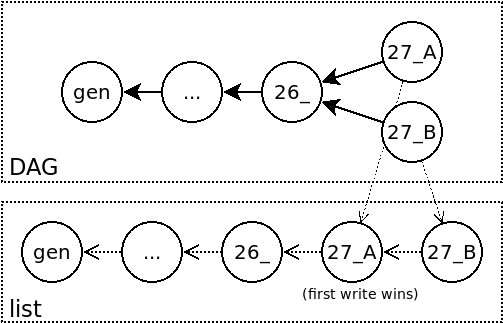
\includegraphics[width=0.35\textwidth]{conflict.png}
\caption{
    The branches in the DAG are ordered by reputation.
    The application ...
}
\label{fig.state}
\end{figure}

Next, we create a conflict situation in which two authors in different peers
edit the same line concurrently:

{\footnotesize
\begin{verbatim}
 # PEER A (more reputation):
 > sed -i 's/peer/Peer/g' p2p.md  # fix typo
 > freechains-vcs #p2p.md commit --sign=699299..
 27_A..

 # PEER B (less reputation):
 > sed -i 's/networking/computing/g' p2p.md
 > freechains-vcs #p2p.md commit --sign=320B59..
 27_B..

 # SYNCHRONIZE (exchange conflicting forks):
 > freechains #p2p.md recv '<our-ip>'
 1 / 1
 > freechains #p2p.md send '<our-ip>'
 1 / 1
 > freechains-vcs #p2p.md checkout p2p.md
 1 out of 1 hunk FAILED -- saving rejects to file p2p.md.rej
 27_B..
 > cat p2p.md
 Peer-to-Peer networking is...
 The [USENET](#usenet.md), ...
 ...
\end{verbatim}
}

After they commit the conflicting changes, the peers synchronize in both
directions and reach the state of Figure~\ref{fig.conflict}.
Then, we checkout the file which applies the patches respecting the consensus
order.
As a result, although the conflict exists, we see that the first branch is
still applied, leaving the file in the longest possible consistent state.
%
Because of the \texttt{break} in the checkout operation above, note that once a
conflict is found, no further patches apply in any of the remaining branches.
%
We chose to adopt a \emph{first write wins} resolution to preserve further work
in the branches with more reputation.
However, the failing patch branch is not totally ignored, since the checkout
saves the conflict file and indicates the block causing it.
%
We believe this optimistic choice is the most advantageous, because it keeps
the file in an usable state while showing that there is a conflict to solve.
For instance, the authors can later decide to dislike one of the two commits to
settle the file and remove the warning.

In summary, the proposed reputation and consensus mechanism empowers a simple
P2P VCS with cooperative authoring and automatic conflict resolution.
It only requires \emph{diff \& patch} and the basic API of \FC with no extra
manipulation of the internal structure of the DAG.

\subsection{Discussion}

In the VCS example, we apply the three-layered CRDT framework discussed in the
beginning of this section as follows:
The whole file commit history of small patches is transported as a DAG between
the peers with the basic commands of \FC.
Eventually, all peers reach to same state with the full commit history.
However, in order to recreate the file, the peers need to interpret the DAG,
which requires a commutative operation because of existing branches.
The \emph{patch} tool is mostly commutative, except for

no need to see the internal structure of the chain dag
only consensus
simple 



Keeping the history, withouth interpreting it, does not raise any conflicts

where else can we use this?
    - reddit
branch contamination


 Since no operations 

of commits
as a last resort

- discutir idempot, comut, assoc
    - merkle vs ops

- converge to same data
    - conflicts are solved
    - or forked w/o breaking
- trivially CRDT as it holds everything
    - except for merges
- but reputation system can help here
    - more reputation applied first
        - conflicts ignored but returned
    - dislikes can clean conflict or even invert if problem is in richest branch

- three levels
    - transport
        - no semantics
    - consensus
        - reputation semantics, much richer than merkle, application can take adv as Git example
        - permanent partition
        - but both working and even communicating (inefficient though)
    - application
        - no guarantees
        - also reordering

- Users can fork or recreate the chain.
  Unlike bitcoin, the value is not on the size, but the cohesion is users.
- Safe for niche topics and minority groups                                     
- Permission less not in the sense that anyone can participate, but more in the sense that content not identity must be verified
- Fulfill the expectations of part of the community                             
- Part from the principle that the pioneers want it to decentralize, otherwise would create a public identity chain fig2


\begin{comment}

\subsection{TODO}

- INSIGHT
 Uso descentralizado
 Emissão descentralizada e restrita
 Criação difícil / Verificação fácil

- users that work twice, bots

Terminar com "@!xxx" dizendo que vale reps mas que owner pode "intervene"

- summary
    - parallel w/ bitcoin
        - ponte entre reputacao -> sybil -> consenso
    - no problem w/ forks

We reach a similar solution to Bitcoin but adapted to our domain
- we need consensus to make the reputation system work
- we need reputation system to reach consensus
- same virutous cycle as bitcoin

The more CPU work is done, the stronger becomes the proposal, the more peers
follow it, the more tokens are mined.
There is a strong association between work, profit and consensus that enables
Bitcoin as a peer-to-peer cash system.

- reputation system to rate messages
    - positively (to distinguish from excess), or
    - negatively (to block SPAM, fake news, illegal content)
- some sort of scarcity (work)
    - you like you loose
    - you work you get
    - otherwise sybil, "likes" abuse
    - incentives for continuous, good quality posts
- consensus to ???

\section{Related Work}
\label{sec.related}

radicle
gun
orbitdb
hypercore

https://ieeexplore.ieee.org/document/5766541
https://arxiv.org/abs/2001.02962

- automerge
Thus, CRDTs have some similarity to version control systems like Git, except that they operate on richer data types than text files. CRDTs can sync their state via any communication channel (e.g. via a server, over a peer-to-peer connection, by Bluetooth between local devices, or even on a USB stick).

Bitcoin employs CPU proof-of-work as a solution, but did not solve the
centralization issue completely because the cost to perform work is not
equally distributed
(depends on costs of equipment and energy)
    - bitcoin demands connectivity to avoid forks
    - forks ok in freechains since operations are not critical and can be reverted
    - 50+1 attack easy in first nodes if not all nodes keep participating
        - freechains requires checkpoints

- related work public forums in scuttlebutt are permissioned (you decide who
  participates). each user has a completely different view of \#chat. not really
  public although some intersections
    - you can see an answer but not a question, or a question w/ no answers
      even if the best answer exists. no content discovery



\section{Conclusion}
\label{sec.conclusion}


Like \emph{bitcoins}, \reps are scarce, hard to generate, and easy to verify.
Unlike \emph{bitcoins}, \reps .


With this design, we retarget  , the balance between work, profit and consensus also applies 

attack 50+1 but not as
cite local-first software

 (crypto proof \& authoring),
while verification is cheap


requires work but evaluation


, but
are evaluated by other user
The system also imposes incentives to rate posts and 

Unlike bitcoin

Since likes and dislikes spend reputation, \emph{creps} are scarce resources
Incentives to post and rate content.

There is a strong association between work, profit and consensus that enables
Bitcoin as a peer-to-peer cash system.

distinguish SPAM from legitimate
Another problem CPU



content.



 (e.g., posts on social media, public conversations
based on the reputation of users
in the network.


biggest difference:
work is subjective as is the evaluation by other users


 with consensus since
whoever proposes the ordering will choose one of the operations arbitrarily


 which is similar to the
example above (\emph{buy X} vs \emph{buy Y})

spent

with work



this gives consensus with total order, solves double spend, which is equivalent
to solving X/Y is decided above

we borrow token, scarcity


 that requires work to 
Only one purpose


- incentive
- security

- Last-Write-Wins

- just all tokens are the same, no subjective judgment, for example on why token is being transferred


 and xx timestamps.


 of the service and , and trust from users to deal

In a decentralized setting, 
    - spam
    - abuse
    - on topic
    - disconnections
    - order

Bitcoin

responses would




n user posts 

- discovery
- also consensus, ensure that participants receive all data in a consistent order
- bitcoin, discovery even disconnected, consensus, but not quality


Regardless of the Internet growth over the years,

\section{Conclusion}
The conclusion goes here.

\end{comment}

\bibliographystyle{IEEEtran}
\bibliography{tpd-21}

\begin{IEEEbiography}{Michael Shell}
Biography text here.
\end{IEEEbiography}

\begin{IEEEbiographynophoto}{John Doe}
Biography text here.
\end{IEEEbiographynophoto}

\begin{IEEEbiographynophoto}{Jane Doe}
Biography text here.
\end{IEEEbiographynophoto}

\end{document}
